\chapter{开发环境及其简介}
\section{开发环境}

以下为开发环境列表
\begin{center}
  \begin{tabular}{lcc}
    \hline
    开发环境 & 名称 & 版本 \\
    \hline
    开发系统 & macOS Big Sur & 11.5.1\\
    IDE & PyCharm & 2021.2\\
    前端 & Vscode & 1.60.1 (Universal)\\
    Python & Python & 3.7.1\\
    Python依赖 & flask, requests, pymysql &  --- \\
    数据库 & MySQL & 8.0.26 Homebrew\\
    \hline
  \end{tabular}
\end{center}

\section{开发环境简介}

% \begin{figure}[htbp]
%   \centering
%   \includegraphics[height=6.0cm,width=9.5cm]{Img/t2.png}%fig2文件夹下的xbee.esp图片,
%   \caption{Campus environment detection system}
% \end{figure}
Flask是一个使用 Python 编写的轻量级 Web 应用框架,包括Werkzeug和Jinja2两个核心函数库,它们分别负责业务处理和安全方面的功能,这些基础函数为web项目开发过程提供了丰富的基础组件。。其 WSGI 工具箱采用 Werkzeug ,模板引擎则使用 Jinja2 ,Flask使用 BSD 授权。Flask的基本模式为在程序里将一个视图函数分配给一个 URL,每当用户访问这个URL时,系统就会执行给该URL 分配好的视图函数,获取函数的返回值并将其显示到浏览器上,其工作过程如下所示。\citep{grinberg2018flask}

\begin{figure}[H]
  \centering
  \includegraphics[width=0.8\textwidth]{t2}
  \bicaption{Flask工作流程}{Flash workflow}
  \label{fig:t2}
\end{figure}


默认情况下,Flask 不包含数据库抽象层、表单验证,或是其它任何已有多种库可以胜任的功能。然而,Flask 支持用扩展来给应用添加这些功能,如同是 Flask 本身实现的一样。众多的扩展提供了数据库集成、表单验证、上传处理、各种各样的开放认证技术等功能。Flask 也许是“微小”的,但它已准备好在需求繁杂的生产环境中投入使用。\citep{赵娟2020浅谈时空大数据与数据可视化在疫情地图中的应用}其特色有如下:

\begin{itemize}
  \item 内置开发用服务器和调试器
  \item 集成的单元测试支持
  \item RESTful请求分派
  \item 使用Jinja2模板引擎
  \item 支持安全cookie(客户端会话)
  \item WSGI1.0兼容
  \item 基于Unicode
  \item 详细的文件、教学
  \item Google App Engine兼容
  \item 可用Extensions增加其他功能
\end{itemize}



